\documentclass[]{beamer}
\usepackage{mathptmx}
\usepackage{graphicx}
\usepackage{parskip}
\usepackage{verbatim}
\usepackage{listings}
\usepackage{dtsyntax}
\usepackage[english]{babel}
\usepackage[utf8]{inputenc}
\usepackage{booktabs}
\usepackage{float}
\usepackage{ulem}
\usepackage{color}
\usepackage{multirow}
\usepackage{lipsum}
\usepackage{epstopdf}
\usepackage{bm}
\newcommand{\cond}{\mathbf{cond}}

\newcommand\gsout{\bgroup\markoverwith
{\textcolor{green}{\rule[3.1pt]{2pt}{1pt}}}\ULon}

%%%%%%%%%% Regler Beamer themes %%%%%%%%%%%%%%%%%
%\usepackage[lionbackground]{beamerthemeRegler}
%\usepackage[lioncorner]{beamerthemeRegler}
%\usepackage[lionheader]{beamerthemeRegler}
\usetheme[lionheader]{Regler}
%%%%%%%%%%%%%%%%%%%%%%%%%%%%%%%%%%%%%%%%%%%%%%%%%

% Title page
\title{Implicit vs. explicit ODE}
\author{Fredrik Magnusson\inst{1} \and Karl Berntorp\inst{2}}
\institute
{
\inst{1} Department of Automatic Control \\
Lund University, Sweden \\
\vspace{14pt}
\inst{2} Mitsubishi Electric Research Laboratories \\
Cambridge, MA \\
\vspace{14pt}
\insertdate
}
\date{November 18, 2015}


% Slide numbering
\definecolor{FootGrey}{RGB}{83,121,170}
\setbeamercolor{foot}{fg=FootGrey,bg=white}
\setbeamertemplate{footline}{
    \begin{beamercolorbox}[right, sep=2.5pt]{foot}
        \insertframenumber{} / \inserttotalframenumber
    \end{beamercolorbox}
}

\begin{document}

{
\setbeamertemplate{footline}{}
\begin{frame}[noframenumbering]
    \titlepage
\end{frame}
}

\begin{frame}
\frametitle{Review}
Last time:
\begin{itemize}
\item
Problem does not seem almost high index
\begin{itemize}
\item
Even if it did, variable scaling should solve the problem
\end{itemize}
\item
Test snow
\end{itemize}
\end{frame}

\begin{frame}
\frametitle{Preview}
This time:
\begin{itemize}
\item
Proper absolute tolerances solves everything
\item
Still some open questions, including optimization
\end{itemize}
\end{frame}

\begin{frame}[fragile]
\frametitle{Absolute tolerance}
\begin{itemize}
\item
Previously used \verb|atol = rtol|
\item
Model contains decent nominal values \verb|nom| for all variables
\item
Instead use \verb|atol = 10*nom*rtol|
\end{itemize}
\end{frame}

\begin{frame}
\frametitle{Simulation results}
Radau5 is reference solution, others have same accuracy

{\small
\begin{table}
\centering
\begin{tabular}{lcc}
\toprule
Setup & tol & Steps [1000] \\
\midrule
Radau5 DAE & 1e-14 & 4.3 \\
IDA DAE & 1e-7 & 2.2 \\
IDA DAE sup. alg. & 1e-8 & 2.0 \\
IDA DAE par. & 1e-7 & 2.0 \\
IDA DAE par. sup. & 1e-8 & 2.2 \\
IDA ODE & 1e-8 & 2.3 \\
\bottomrule
\end{tabular}
\end{table}
}

Conclusion: Algebraic error control was running amok due to unreasonable tolerances for algebraics
\end{frame}

\begin{frame}
\frametitle{Iteration matrix condition number}
Consider
\begin{align*}
F(\dot x, x, y) &= 0 \\
G(x, y) &= 0
\end{align*}
\begin{itemize}
\item
BDF iteration matrix:
\begin{equation}
J = \begin{bmatrix}
\frac{\alpha_0}{h} \nabla_{\dot x}F + \nabla_x F & \nabla_y F \\
\nabla_x G & \nabla_y G
\end{bmatrix}
\end{equation}
\item
(Theorem 5.4.1) Condition number of iteration matrix is $\mathcal{O}(h^{-\nu})$
\item
Conjecture: If $\nabla_{\dot x}F = I$ and first row of $J$ is scaled by $h$, condition number is instead $\mathcal{O}(h^{-\nu-1})$
\begin{itemize}
\item
What to do if $\nabla_{\dot x}F$ is not square? What does IDA do?
\item
Maybe I should do something like this in my collocation implementation?
\end{itemize}
\end{itemize}
\end{frame}

\begin{frame}
\frametitle{Condition number}
\begin{columns}
\column{0.5\linewidth}
\centering
DAE
\begin{figure}[ht]
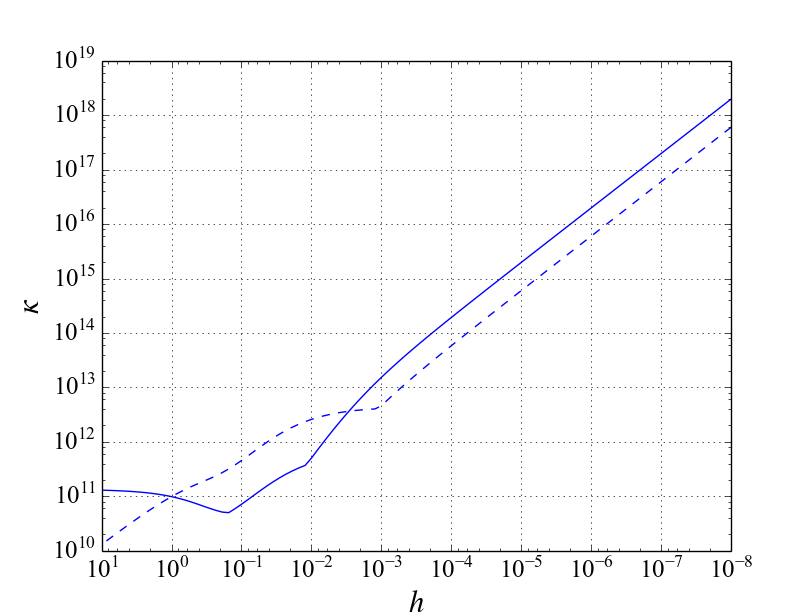
\includegraphics[width=\linewidth]{dae_cond.png}
\end{figure}

\column{0.5\linewidth}
\centering
ODE
\begin{figure}[ht]
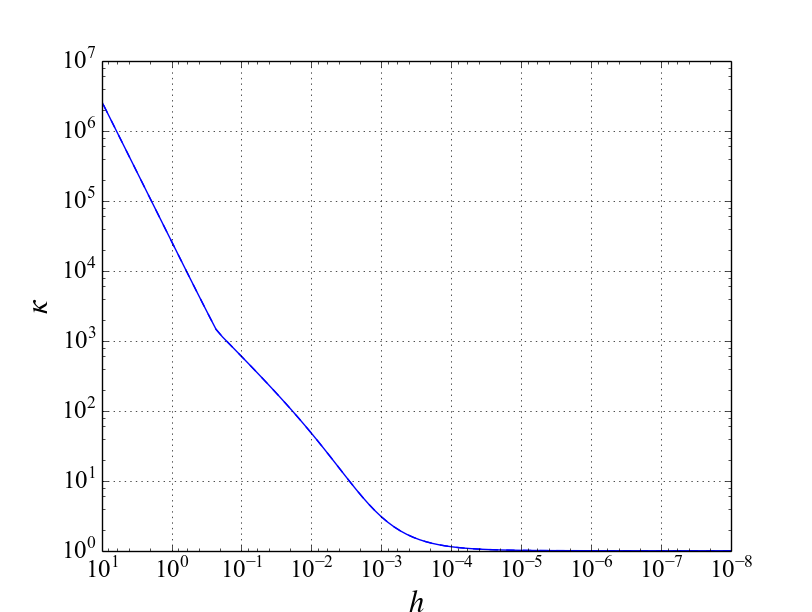
\includegraphics[width=\linewidth]{ode_cond.png}
\end{figure}
\end{columns}
\end{frame}

\begin{frame}
\frametitle{Commutativity}
\begin{itemize}
\item
Previously: Does BLT and fixed-step collocation commute?
\item
Consider single integration step of
\begin{equation}
\begin{aligned}
\dot x &= f(x, y, u) \\
y &= g(x, u),
\end{aligned}
\end{equation}
and
\begin{equation}
\dot x = f(x, g(x, u), u)
\end{equation}
\end{itemize}
\end{frame}

\begin{frame}
\frametitle{Commutativity}
Explicit DAE:
\begin{subequations}
\begin{gather}
\dot x_k = f(x_k, y_k, u_k), \\ 
y_k = g(x_k, u_k), \\
\dot{x}_k = \frac{1}{h} \cdot \sum_{n = 0}^{n_c} \alpha_{n, k} x_n, \\
\forall k \in [1 . . n_c]
\end{gather} 
\end{subequations}

Explicit ODE:
\begin{subequations}
\begin{gather}
\dot x_k = f(x_k, g(x_k, u_k), u_k), \\ 
\dot{x}_k = \frac{1}{h} \cdot \sum_{n = 0}^{n_c} \alpha_{n, k} x_n, \\
\forall k \in [1 . . n_c]
\end{gather} 
\end{subequations}

Clearly commutative?
\end{frame}

\begin{frame}
Bilevel control: Single-track used on high level to generate reference trajectory, double-track used on low level to follow trajectory
\frametitle{MPC}
\begin{columns}
\column{0.5\linewidth}
\begin{figure}[ht]
\centering
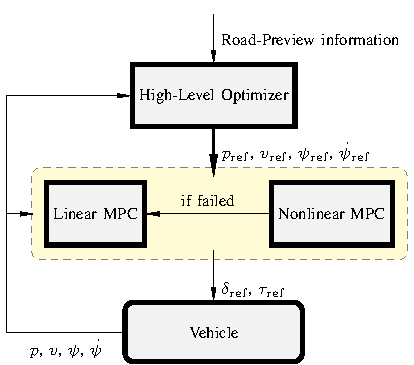
\includegraphics[width=\linewidth]{structure.pdf}
\end{figure}

\column{0.5\linewidth}
\begin{figure}[ht]
\centering
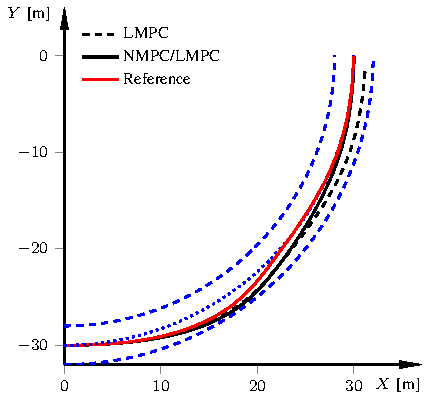
\includegraphics[width=\linewidth]{mpcxy.pdf}
\end{figure}
\end{columns}
\end{frame}

\begin{frame}
\frametitle{Convergence}
\begin{itemize}
\item
High level needs to be solved over free time horizon $\implies$ difficult
\item
Low level has fixed time horizon (MPC) $\implies$ less difficult
\item
Newton's method does not converge at all for high-level problem if we use full DAE, but converges for ODE
\item
Usually converges for low level even with DAE, but ODE more robust and faster
\end{itemize}
\end{frame}

\begin{frame}
\frametitle{High level}
Will today focus on high-level problem:
\begin{equation}
\begin{aligned}
	\underset{\delta_\mathrm{ref},\tau_{f,\mathrm{ref}},\tau_{r,\mathrm{ref}}}{\mathrm{minimize}} & \quad \int_{t_0}^{t_f}\!(\kappa_1 e^2 + \kappa_2\beta^2) \,\mathrm{d}t  \\
	\underset{\phantom{\delta_\mathrm{ref},\tau_{f,\mathrm{ref}},\tau_{r,\mathrm{ref}}}}{\mathrm{subject \ to}} & \quad    |\tau_{i,\mathrm{ref}}|
     \leq \tau_{i,\mathrm{max}}, \ \forall i \in \{f,r\}, \\[-10pt]
& \quad |\delta_\mathrm{ref}| \leq \delta_{\mathrm{max}},  \\
& \quad \lVert p(t_f)-p_{t_f}\rVert\leq \epsilon,\\
&           \quad \Gamma(p) \leq 0, \quad x(t_0) = x_0, \\
	& \quad F(\dot x,x,y,\delta_\mathrm{ref},\tau_{f,\mathrm{ref}},\tau_{r,\mathrm{ref}}) = 0
\end{aligned}
\end{equation}
\end{frame}

\begin{frame}
\frametitle{Dynamic optimization}
More abstract/compact formulation ($\bm z := (\dot{\bm x}, \bm x, \bm y, \bm u)$):
{\small
\begin{subequations}\label{eq:DOP}
\begin{alignat}{3}
& \text{minimize \hspace{10pt}} && \int_{t_0}^{t_f} L(\bm z(t))\,\mathrm{d}t \label{eq:DOP!objective}, && \\
& \text{with respect to \hspace{10pt}} && \bm x : [t_0, t_f] \rightarrow \mathbb{R}^{n_x}, && \bm y : [t_0, t_f] \rightarrow \mathbb{R}^{n_y}, \nonumber \\
&&& \bm u : [t_0, t_f] \rightarrow \mathbb{R}^{n_u}, && t_f \in \mathbb{R}, \nonumber \\
& \text{subject to \hspace{10pt}} && \bm F(\bm z(t)) = \bm 0, &\quad& \bm F_0(\bm z(t_0)) = \bm 0, \label{eq:DOP!dynamics}\\
&&& \bm z_L \leq \bm z(t) \leq \bm z_U, \\
&&& \bm g(\bm z(t)) \leq \bm 0, &\quad& \bm G(\bm z(t_f)) \leq \bm 0, \label{eq:DOP!path_constraints} \\
&&& \forall t \in [t_0, t_f]. && \nonumber
\end{alignat}
\end{subequations}
}
\end{frame}

\begin{frame}
\frametitle{NLP}
{\small
Discretize differential equations to get a finite-dimensional nonlinear program (NLP) ($\bm z_{i, k} \approx \bm z(t_{i, k})$, where $t_{i, k}$ is collocation point $k$ in element $i$):
}
\vspace{-4pt}
{\small
\begin{subequations}
\begin{alignat}{3} 
& \text{minimize } && \rlap{$\displaystyle\sum_{i = 1}^{n_e} h_i \cdot (t_f - t_0) \cdot \sum_{k = 1}^{n_c} \omega_k \cdot L\left(\bm z_{i, k}\right)$,} \label{eq:DOP_NLP!objective} \\
& \text{with respect to \hspace{5pt}} && \rlap{$\bm z_{i, k} \in \mathbb{R}^{2n_x + n_y + n_u}, \quad \bm x_{i, 0} \in \mathbb{R}^{n_x}, \quad t_f \in \mathbb{R}$,} \nonumber \\  
& \text{subject to } && \bm F(\bm z_{i, k}) = \bm 0, &\quad& \bm F_0(\bm z_{1, 0}) = \bm 0 \label{eq:DOP_NLP!dynamics}, \\ 
&&& \bm u_{1, 0} = \sum_{k = 1}^{n_c} \bm u_{1, k} \cdot \ell_k(0) &\quad& \bm z_L \leq \bm z_{i, k} \leq \bm z_U, \label{eq:DOP_NLP!bounds} \\ 
&&& \bm g(\bm z_{i, k}) = \bm 0, &\quad& \bm G(\bm z_{n_e, n_c}) \leq \bm 0, \label{eq:DOP_NLP!point_constraints} \\
&&& \rlap{$\forall (i, k) \in \{(1, 0)\} \cup ([1 . . n_e] \times [1 . . n_c]),$} \nonumber \\ 
&&& \rlap{$\displaystyle\dot{\bm x}_{j, l} = \frac{1}{h_j \cdot (t_f - t_0)} \cdot \sum_{m = 0}^{n_c} \bm x_{j, m} \cdot \frac{\mathrm{d}\tilde{\ell}_m}{\mathrm{d}\tau}(\tau_l),$} \\ &&& \forall (j, l) \in [1 . . n_e] \times [1 . . n_c], \\ 
&&& \rlap{$\bm x_{n, n_c} = \bm x_{n+1, 0}, \quad \forall n \in [1..n_e-1].$} \label{eq:DOP_NLP!continuity} 
\end{alignat}
\end{subequations}
}
\end{frame}

\begin{frame}
\frametitle{NLP solution}
After further abstraction, the NLP is:
\begin{subequations}
    \begin{alignat*}{2}
        & \text{minimize } && f(x), \\
        & \text{with respect to \hspace{5pt}} && x \in \mathbb{R}^m, \\
        & \text{subject to } && x_L \leq x \leq x_U, \\
        &&& g(x) = 0, \\
        &&& h(x) \leq 0.
    \end{alignat*}
\end{subequations}
\begin{itemize}
\item
Solved by IPOPT
\item
Lots of complicated details, but essentially Newton's method is applied on KKT optimality conditions
\item
See bonus slides for details
\end{itemize}
\end{frame}

\begin{frame}
\frametitle{Convergence}
Why convergence issues are more prominent in optimization than simulation in general:
\begin{itemize}
\item
Larger system of equations (dual variables + TBVP)
\item
No good initial guess (at least not for high-level problem)
\item
Inherently ill-conditioned (see bonus slides)
\end{itemize}
\end{frame}

\begin{frame}
\frametitle{Restoration phase}
\begin{itemize}
\item
For the high-level problem, IPOPT fails in restoration
\item
Restoration is triggered for various reasons, but usually because of ill-conditioned Jacobian
\item
Restoration means that IPOPT stops solving the optimization problem and instead solves
\begin{subequations}
    \begin{alignat*}{2}
        & \text{minimize } && ||g(x)||_1 + ||h(x) - y||_1 + 0.5\zeta||D_R(x-x_R)||_2^2, \\
        & \text{with respect to \hspace{5pt}} && x \in \mathbb{R}^m, \quad y \in \mathbb{R}^n\\
        & \text{subject to } && x_L \leq x \leq x_U, \\
        &&& y \leq 0.
    \end{alignat*}
\end{subequations}
\item
IPOPT finds a local minimum to this problem which is not feasible; failure
\end{itemize}
\end{frame}

\end{document} 